
%\newpage
%\blankpage

\chapter{Presentaciones de grupos} \label{pg}

%Definición axiomatizada, donde se debe comprobar la asociatividad, existencia de elemento neutro y existencia de elemento inverso para cada elemento, \ref{defgrupo}.


%En ejemplos de grupos de orden pequeño no supone un problema numerar los elementos, sin embargo, no ocurre lo mismo cuando el orden del grupo es grande.
Actualmente, un \textit{grupo abstracto} debe satisfacer la Definición \ref{defgrupo}. Sin embargo, podemos describir el grupo y sus elementos de dos formas:

\begin{enumerate} \label{haydos}
    \item Enumerando los elementos del grupo junto a la operación binaria, de igual modo que se han dado en el Ejemplo \ref{ejemplosgr} anterior. %, \ref{defgrupo}.
    \item En términos de generadores y relatores. En secciones anteriores se han introducido grupos como el grupo Diédrico $D_n$ o el grupo de los Cuaternios $Q_2$, cuyos elementos satisfacen una serie de propiedades.

El grupo $D_n$ está generado por $\varphi$ y $\sigma$, que cumplen: 
\begin{align*} \label{alli}
    \varphi^n=1, \quad \sigma^n=1, \quad \sigma \varphi = \varphi^{-1}\sigma \:.
\end{align*}

En el caso de $Q_2$, podemos generalizar el grupo y obtener el grupo generalizado de los Cuaternios $Q_n$, de forma que sus elementos cumplan las siguientes relaciones:
\[
    x^{2n}=1, \quad x^n=y^2 \quad e \quad yxy^{-1}=x^{-1} \:.
\]

Por ello, podemos pensar en presentar un grupo como un conjunto de generadores $S$ de $G$ y un conjunto de relatores $R$ que los elementos de $S$ deben satisfacer para determinar $G$.  Esto es lo que se conoce como \textit{presentación de un grupo} y se precisará en esta sección. Para llevar a cabo esto, necesitamos introducir primero el concepto de \textit{grupo libre}. La documentación usada para esta sección ha sido principalmente ~\cite{free} e ~\cite{carlos}.
    
\end{enumerate}


\section{Grupo libre}

Sea X un conjunto arbitrario.  Consideramos el conjunto $X^{\pm 1} = X^{+1} \cup X^{-1}$ donde cada elemento $x\in X$ tendrá un elemento  $x^{+1}\in X^{+}$ y otro asociado $x^{-1} \in X^{-1}$. Para simplificar notación, identificamos $X^{+1}$ con $X$.

Una \textit{palabra} en $X$ es una secuencia finita de elementos
\begin{equation}\label{eq1}
     w=x_{a_1}^{\epsilon_1} x_{a_2}^{\epsilon_2} \cdots x_{a_n}^{\epsilon_n} \quad \text{con } x_{a_i} \in X, \hspace{0.2cm} \epsilon_i \in \{+ 1, -1\},
     \: n \in \mathbb{N}; %, \hspace{0.2cm} i \in \{1,\ldots,n\}
    % epsilon podría valer también 0 
\end{equation}

y será \textit{reducida} si no contiene subpalabras del tipo $xx^{-1}$ o $x^{-1}x$  . %ni 1. 
Por otro lado, su longitud estará determinada por el número de elementos que contiene, $|w|=n$. Asumimos que la palabra vacía, $\epsilon$, es reducida, luego $|\epsilon|=0$. 


Si $G$ es un grupo y $X\subseteq G$, una palabra de $G$ en $X$ es una expresión $w$ como en \eqref{eq1} en la que yuxtaposición indica producto y $^{-1}$ indica inverso.

\begin{definition} 
Un subconjunto $X$ de un grupo $G$ es un sistema de generadores si todo elemento de $G$ se puede escribir como una palabra (reducida) en $X$.
\end{definition}


\begin{remark}
Todo grupo tiene un sistema de generadores, basta con tomar el propio grupo como conjunto.
\end{remark}

\begin{definition}
Diremos que los elementos de un subconjunto $X\subseteq G$ son independientes si la única palabra reducida en $X$ que es igual a $1\in G$ es la palabra vacía.
\end{definition}

\begin{definition}
Un grupo $G$ es libre si tiene una base, esto es, si existe un subconjunto $X$ de elementos independientes que son un sistema de generadores, donde cada palabra reducida no vacía en $X^{\pm 1}$ define un elemento no trivial en $G$. Llamamos rango de un grupo libre al cardinal de cualquiera de sus bases.
\end{definition}


%\begin{remark}
%En este contexto, X se denominará una \textit{base libre} de G y G será \textit{libre} en X. Además, diferentes palabras reducidas en X definirán diferentes elementos en G.
%\end{remark}



Sea $X$ un conjunto arbitrario. Nuestro objetivo ahora es la \textit{``construcción''} de un grupo libre con base $X$. Para ello, se seguirá un proceso de reducción sobre el conjunto de palabras que contiene, en el que se eliminarán subpalabras del tipo $xx^{-1}$ y $x^{-1}x$ hasta obtener un conjunto en el que todas las palabras sean reducidas. Se deberán tener en cuenta las siguientes consideraciones.
\begin{enumerate}
    \item \textbf{El proceso de reducción no es único}: En la clase de equivalencia de una palabra existe una única palabra reducida, aunque puede haber distintos procesos de reducción para obtenerla.
    \[
    \begin{tikzcd}
    & w_1 \arrow[dr,dashrightarrow]{} \\
    w \arrow[r] \arrow[ur] \arrow[dr]  & \ldots \arrow[r,dashrightarrow] & w_n \\
    & w_2 \arrow[ur,dashrightarrow]{}
    \end{tikzcd}
    \]
    \item \textbf{Palabras equivalentes}: Diremos que dos palabras son equivalentes si podemos pasar de una a otra por un proceso de reducción.
\end{enumerate}


%Sea X un conjunto arbitrario. Nuestro objetivo ahora es la 'construcción' de un grupo libre con base X. Para ello, se seguirá un proceso de reducción en el que se eliminarán subpalabras del tipo $xx^{-1}$ y $x^{-1}x$ hasta obtener un conjunto en el que todas las palabras estén reducidas. En general, puede haber diferentes reducciones para una misma palabra $w$, sin embargo, todas estas posibles reducciones dar lugar a la misma palabra reducida.
%¿Quizás repito mucho "reducir" ?

%\begin{enumerate}
 %   \item \textcolor{red}{Diremos que dos palabras son equivalentes si podemos pasar de una a otra por un proceso de reducción.}
 %   \item \textcolor{red}{En la clase de equivalencia de una palabra existe una única palabra reducida, aunque haya distintos procesos de reducción para obtenerla}
%\end{enumerate}




Dado un conjunto $X$, denotamos por $\operatorname{F}(X)$ al conjunto de sus palabras reducidas.
%\textcolor{red}{Dado un conjunto $X$ denotaremos $F(X)$ al conjunto de las palabras reducidas en $X$}.


A partir de dos palabras reducidas, $w_1$ y $w_2$, podemos definir su \textbf{producto} como la única palabra reducida en la clase de la palabra que se obtiene por concatenación de ambas: \label{producto}
\begin{align*}
\begin{rcases}
w_1 &= x_{a_1}^{\epsilon_1} \cdots x_{a_n}^{\epsilon_n}  \\
w_2 &= x_{b_1}^{\epsilon_1} \cdots x_{b_m}^{\epsilon_n}
\end{rcases}
\end{align*}

Definimos $w_1\cdot w_2$ como la única palabra reducida en la clase de $x_{a_1}^{\epsilon_1} \cdots x_{a_n}^{\epsilon_n} \hspace{0.1cm} x_{b_1}^{\epsilon_1} \cdots x_{b_m}^{\epsilon_m}$; es decir, sobre la concatenación $w_1w_2$ se realiza un proceso de reducción eliminando parejas de elementos asociados si fuera necesario. 

%En la expresión del producto $w_1 \cdot w_2$ anterior se obtiene una nueva palabra reducida eliminando subpalabras si fuera necesario.

%Con esto me refiero a que se eliminan xx^{-1}, x^{-1}x. Diría que no es necesario indicarlo porque se sobreentiende (se ha comentado en el párrafo anterior)



%\begin{remark}
%$X$ es un sistema de generadores de $F(X)$ y cada palabra reducida no vacía en $X^{\pm 1}$ define un %elemento no trivial en $F(X)$. Por lo tanto, $X$ es una base de $F(X)$ o, equivalentemente, $F(X)$ es %libre en $X$.
%\end{remark}

%!!!



\begin{theorem}[Existencia]
%Sea X un conjunto.
El conjunto $\operatorname{F}(X)$ de palabras reducidas en $X$ dotadas con el producto anterior forman un grupo libre con base el conjunto $X$.
\end{theorem}

\begin{proof}
%La operación está bien definida ya que el producto de dos palabras reducidas también lo es. Por otro lado, se tiene:

La operación está bien definida ya que el producto de dos palabras reducidas dotado con el proceso de reducción da lugar a una palabra reducida.
\begin{itemize}
    \item La palabra vacía $\epsilon$ es la identidad.
    \[
        w = \epsilon \cdot w = w \cdot \epsilon \: .
    \]
    \item El elemento inverso de una palabra $w = x_{a_1}^{\epsilon_1} x_{a_2}^{\epsilon_2} \cdots x_{a_r}^{\epsilon_r} $ viene dado por:
    \[w^{-1} = x_{a_r}^{-\epsilon_r} \cdots x_{a_2}^{-\epsilon_2} x_{a_1}^{-\epsilon_1} .
    \]
    \item Veamos que se cumple también la propiedad asociativa, es decir:
    \[
        w_1(w_2w_3)=(w_1w_2)w_3 \:.
    \]
    Realicemos un proceso inductivo sobre la longitud de $w_2$.
    \begin{enumerate}
        \item $|w_2|=1$ (se tiene que $w_2=x$ o $w_2=x^{-1}$, para algún $x\in X$). A partir de esto nos encontramos con las siguientes situaciones: Que el último elemento de $w_1$ sea o no asociado con $w_2$ y que el primer elemento de $w_3$ sea o no asociado con $w_2$.
        En las 4 posibilidades se ve claramente que $w_1(w_2w_3) = (w_1w_2)w_3$.
        
        \item Supuesto cierto para $|w_2|\leq n$, veamos que se cumple para $|w_2|=n+1$.
        
        Sea $w_2=w_k x^{\epsilon}$, donde $\epsilon=\pm 1$ y $x \in X$.
        \begin{align*}
            w_1(w_2w_3) = & w_1((w_kx^{\epsilon})w_3) = (w_1w_k)(x^{\epsilon}w_3) \\ =&((w_1w_k)x^{\epsilon})w_3 = (w_1(w_kx^{\epsilon}))w_3 = (w_1w_2)w_3 \: .
        \end{align*}
    \end{enumerate}
\end{itemize}
\end{proof}

%El conjunto de palabras reducidas en X satisface todos los axiomas de un grupo.




\begin{theorem}[Propiedad Universal del grupo libre]
%Quizás es redundante poner F(X). Con indicar que F es generado por X, basta con poner 'F', no?

%Sea X un conjunto. Un grupo libre F con base X satisface la siguiente propiedad universal:
%Para cualquier grupo G y aplicación $\varphi \colon X  \rightarrow G$ existe un único homomorfismo de %grupos $\varphi^*: F(X) \rightarrow G$ extendiendo $\varphi$, que hace el siguiente diagrama %conmutativo: 
%\[
%\begin{tikzcd}
% X \arrow[r,hook]{}{i} \arrow[dr,']{}{\varphi} & F(X) \arrow[d]{}{\varphi^*}\\
%& G
%\end{tikzcd}
%\]
Sea $\operatorname{F}$ un grupo libre y $X\subseteq \operatorname{F}$ una base de $\operatorname{F}$. Entonces, para cualquier grupo $G$, dar un morfismo de grupos $\varphi^*:F\to G$ es equivalente a dar una aplicación $\varphi:X\to G$. En otras palabras:

\[
\begin{tikzcd}
 X \arrow[r,hook]{}{i} \arrow[dr, ']{}{\forall \varphi \text{ aplicación}} & F \arrow[d,dashrightarrow]{}{\exists !\varphi^* \text{ morfismo}}\\
& G
\end{tikzcd}
\]

%\[
%\begin{tikzcd}
% X \arrow[r,hook]{}{i} \arrow[dr, %']{}{\varphi} & \operatorname{F} %\arrow[d,dashrightarrow]{}{\varphi^*}\\
%& G
%\end{tikzcd}
%\]

\end{theorem}

\begin{proof}


%Como F(X) es libre en X, se tiene que cada elemento $w\in F(X)$ se define por una única palabra reducida en $X^{\pm 1}$,

Como $X$ es base de $\operatorname{F}$, se tiene que cada elemento $w\in \operatorname{F}$ se define por una única palabra reducida en $X^{\pm 1}$,
\[
 w=x_{a_1}^{\epsilon_1} \cdots x_{a_n}^{\epsilon_n} \quad \text{con } x_{a_i} \in X, \hspace{0.2cm} \epsilon_i \in \{+ 1, -1\} \:, n \in \mathbb{N} .
\]

Dado $\varphi$, definimos $\varphi^*$ como:
\begin{align} \label{ant}
    \varphi^*(w) = \varphi^*(x_{a_1}^{\epsilon_1} \cdots x_{a_n}^{\epsilon_n}) = \varphi(x_{a_1})^{\epsilon_1} \cdots \varphi(x_{a_n})^{\epsilon_n}.
\end{align}


donde se ve que claramente $\varphi^*$ es un homomorfismo de grupos y el diagrama conmuta.
%¿Es suficiente con esto? podría tomar dos elementos w1,w2 de F(X) y ver que \varphi*(w1 w2) = \varphi*(w1) \varphi*(w2) pero se ve que sí se cumple.

%Por otro lado, $\varphi^*$ extiende $\varphi$ y el diagrama conmuta. 
Cualquier homomorfismo $\varphi^* \colon \operatorname{F} \rightarrow G$ que haga el diagrama conmutativo debe satisfacer \eqref{ant}, por tanto, $\varphi^*$ es único.
\end{proof}












\begin{theorem}[Unicidad]
 Si $G$ es un grupo libre y $X$ es una base de $G$, entonces $G$ es isomorfo a $\operatorname{F}(X)$.
\end{theorem}

\begin{proof}
Definimos las inclusiones:
\[
    X \xrightarrow[]{ \hspace{0.2cm} \varphi_1 \hspace{0.2cm}} G \: ; \quad X \xrightarrow[]{ \hspace{0.2cm} \varphi_2 \hspace{0.2cm}} F(X) .
\]
Por la propiedad universal de grupos libres, como $X$ es base de $G$ y de $\operatorname{F}(X)$, existirán dos homomorfismos:
\begin{align} \label{arriba}
    \varphi_1^* \colon G \rightarrow \operatorname{F}(X) \hspace{0.2cm} \text{ tal que }  \hspace{0.2cm} \varphi_1^* \circ \varphi_1 = \varphi_2, \\
    \varphi_2^* \colon \operatorname{F}(X) \rightarrow G  \hspace{0.2cm} \text{ tal que }  \hspace{0.2cm} \varphi_2^* \circ \varphi_2 = \varphi_1.
\end{align}

En otras palabras:
\[
\begin{tikzcd}
     X \arrow[rr]{}{\varphi_1} \arrow[dd, ']{}{\varphi_2} && G \arrow[ddll, bend right=-16]{}{\varphi_1^*}\\
     && \\
     \operatorname{F}(X) \arrow[uurr, bend right=-5]{}{\varphi_2^*} 
\end{tikzcd}
\]

La composición $(\varphi_1^* \circ \varphi_2^*) \colon \operatorname{F}(X) \rightarrow \operatorname{F}(X)$ es un homomorfismo que cumple:
\[
    (\varphi_1^* \circ \varphi_2^*) \circ \varphi_2 = \varphi_1^* \circ (\varphi_2^* \circ \varphi_2) = \varphi_1^* \circ \varphi_1 \overset{\mathrm{(\ref{arriba})}}{=} \varphi_2
\]
Análogamente, se tiene que $(\varphi_2^* \circ \varphi_1^*) \circ \varphi_1 = \varphi_1$. Por tanto,  $(\varphi_1^* \circ \varphi_2^*)$ y $(\varphi_2^* \circ \varphi_1^*)$ son, respectivamente, las aplicaciones identidad en $\operatorname{F}(X)$ y $G$, obteniendo así que $G \cong \operatorname{F}(X)$. \end{proof}






\newpage
\begin{theorem}
Si X e Y son dos bases de un grupo libre $\operatorname{F}$, entonces $|X| = |Y|$.
\end{theorem}

\begin{proof}
Por la propiedad universal del grupo libre, cualquier aplicación $X \rightarrow \mathbb{Z}_2$ da lugar a un homomorfismo de $\operatorname{F}$ en el grupo cíclico $\mathbb{Z}_2$. Denotando por $\operatorname{Hom}(\operatorname{F},\mathbb{Z}_2)$ al conjunto de homomorfismos de $\operatorname{F}$ a $\mathbb{Z}_2$, se tiene que $|\operatorname{Hom}(\operatorname{F},\mathbb{Z}_2)|=2^{|X|}$. Esto implica
\[
    2^{|X|} = 2^{|Y|} \: \text{, por lo que } \:  |X|=|Y|.
\]\end{proof}
%En la última implicación, si ambos conjuntos son infinitos se ha de asumir la Hipótesis del Continuo de la teoría de conjuntos.








\begin{theorem} \label{dema}
%Sean X e Y dos conjuntos arbitrarios. 
Dos grupos libres $\operatorname{F}(X)$ y $\operatorname{F}(Y)$ son isomorfos si, y sólo si, $|X|=|Y|$.
%X e Y son conjunto, se entiende que |X| es el cardinal.
\end{theorem}

\begin{proof}
\mbox{}\par 
Suficiencia. Supongamos que $|X|=|Y|$. Como ambos conjuntos tienen la misma cardinalidad, existe una correspondencia uno a uno, a la que llamamos $f$:
\[
    f \colon X \rightarrow Y \quad y \quad f^{-1} \colon Y \rightarrow X .
\]

Como $\operatorname{F}(X)$ y $\operatorname{F}(Y)$ son grupos libres, el teorema universal de grupos libres nos garantiza la existencia de únicos homomorfismos $\varphi$ y $\varphi^{-1}$ que extienden a $f$ y $f^{-1}$.
Por tanto:
\[
    \varphi \colon \operatorname{F}(X) \rightarrow \operatorname{F}(Y) \quad y \quad \varphi^{-1} \colon \operatorname{F}(Y) \rightarrow \operatorname{F}(X) .
\]
La composición $(\varphi \circ \varphi^{-1}) \colon \operatorname{F}(X) \rightarrow \operatorname{F}(X)$ extiende la identidad en X. De igual forma, $(\varphi^{-1} \circ \varphi)\colon \operatorname{F}(Y) \rightarrow \operatorname{F}(Y)$ extiende la identidad en Y. Así, $\operatorname{F}(X)\cong \operatorname{F}(Y)$.



Necesidad. Supongamos ahora que $\operatorname{F}(X) \cong \operatorname{F}(Y)$. Consideremos el conjunto de homomorfismos de $\operatorname{F}(X)$ a $\mathbb{Z}_2$ y de $\operatorname{F}(Y)$ a $\mathbb{Z}_2$, denotados por $\operatorname{Hom}(\operatorname{F}(X),\mathbb{Z}_2)$ y $\operatorname{Hom}(\operatorname{F}(Y),\mathbb{Z}_2)$, respectivamente. Como $\operatorname{F}(X) \cong \operatorname{F}(Y)$, se tendrá que:
\[
|\operatorname{Hom}(\operatorname{F}(X),\mathbb{Z}_2)| = |\operatorname{Hom}(\operatorname{F}(Y),\mathbb{Z}_2)|
\]
y, por definición de grupo libre, habrá tantos homomorfismos de $\operatorname{F}(X)$ en $\mathbb{Z}_2$ como aplicaciones de X en $\mathbb{Z}_2$. Análogo para $\operatorname{F}(Y)$ e Y, luego:
\[
    2^{|X|} = |\operatorname{Hom}(\operatorname{F}(X),\mathbb{Z}_2)| = |\operatorname{Hom}(\operatorname{F}(Y),\mathbb{Z}_2)| =  2^{|Y|} ,
\]
lo cual implica que $ |X|=|Y|$.
\end{proof}



Como consecuencia del Teorema \ref{dema}, salvo isomorfismo hay sólo un grupo libre de un rango dado. Como norma general, $\operatorname{F}_n$ representa \textbf{el} grupo libre de rango $n$, salvo isomorfismos.
%Además, todas las bases de un grupo libre F tienen el mismo cardinal.





%\begin{theorem}
%Todo grupo $G$ es isomorfo a un cociente de un grupo libre.
%\end{theorem}
%
%\begin{proof}
%Consideremos G visto como conjunto y la aplicación:
%\begin{align*}
%    Id_G \colon G &\rightarrow G \\
%    x &\mapsto x , \quad \forall x \in G
%\end{align*}
%
%Por ser $F(G)$ un grupo libre sobre $G$, existirá un único homomorfismo:
%\[
%    \varphi \colon F(G) \rightarrow G
%\]
%que hace conmutativo al diagrama
%\[
%\begin{tikzcd}
% G \arrow[r,hook]{}{i} \arrow[dr]{}{Id_G} & F(G) \arrow[d]{}{\varphi}\\
%& G
%\end{tikzcd}
%\]
%es decir, $\forall x \in G$ se tiene:
%\[
%    \varphi \circ i (x) = Id_G(x) = x
%\]
%Por tanto, $\varphi$ es un epimorfismo %homomorfismo sobreyectivo
%y, aplicando el Primer Teorema de Isomorfía, 
%\[
%    G \cong F(G)/ker(\varphi)
%\]
%\end{proof}









\newpage
\begin{theorem}\label{coli}
Todo grupo es isomorfo a un cociente de un grupo libre.
\end{theorem}

\begin{proof}
%Sea G un grupo con un conjunto generador X.
Sea $G$ un grupo y $X$ un sistema de generadores de $G$.


%Por la propiedad universal de grupos libres existe un homomorfismo:
Consideremos $\operatorname{F}(X)$ el grupo libre sobre $X$, la inclusión $X\hookrightarrow G$ induce, por la propiedad universal del grupo libre, un homomorfismo:
\[
    \varphi \colon \operatorname{F}(X) \rightarrow G \text{ tal que }  \varphi(x)=x, \:  \text{para todo } x \in X. 
\]
que hace conmutativo al diagrama:
\[
\begin{tikzcd}
 X \arrow[r,hook]{}{i} \arrow[dr,']{}{i} & \operatorname{F}(X) \arrow[d]{}{\varphi}\\
& G
\end{tikzcd}
\]

El homomorfismo $\varphi$ es sobreyectivo porque es la aplicación identidad en $X$, luego aplicando el primer Teorema de Isomorfía,
\[
    G = \operatorname{Im}(\varphi) \cong \operatorname{F}(X)/\operatorname{ker}(\varphi). %= \langleX|ker(\varphi) \rangle 
\]
\end{proof}
%y así, podemos afirmar que todo grupo tiene una presentación. 


%En este contexto, una palabra $w\in ker(\varphi)$ es un \textit{relator} y $ker(\varphi)$ es el conjunto de relatores de G. Si un subconjunto $R \subseteq ker(\varphi)$ genera $ker(\varphi)$ como subgrupo normal de F(X), entonces se denomina \textit{conjunto de relaciones} de G. 


%El par $\langleX|R \rangle $ se conoce por \textit{presentación}, y determina G unívocamente (salvo isomorfismos).
%La presentación $\langleX | R \rangle $ será finita siempre que lo ambos conjuntos X y R también lo sean y un grupo será presentado de forma finita si tiene al menos una presentación finita.



%Indicar también algo sobre el rango, para cuando estés con presentaciones puedas asegurar que si el grupo es finitamente generado, entonces se pueden obtener un número finito de relatores.
\begin{theorem}[Nielsen-Schreier]\label{niel}
Todo subgrupo de un grupo libre es libre.
Además, si $\operatorname{F}$ es libre de rango $n$ todo subgrupo suyo es libre de rango menor o igual a $n$.
\end{theorem}
La demostración requiere de conceptos topológicos que no serán estudiados por lo que se puede consultar ~\cite{Nielsen} para una descripción detallada.

%https://core.ac.uk/download/pdf/229960372.pdf









\newpage 
\section{Presentación de un grupo}



En el Teorema \ref{coli} se ha probado que todo grupo $G$ es isomorfo a un cociente de un libre:
\[
    G \cong \operatorname{F}(X)/K ,
\]
donde $\varphi \colon \operatorname{F}(X) \twoheadrightarrow G$ es un epimorfismo y $K=ker(\varphi) \trianglelefteq G$, un subgrupo normal. 
Como X es un sistema de generadores de $G$, aplicando el Teorema \ref{niel}, se tiene que K es libre y podremos tomar $R\subseteq K$ una base de $K$. 

Los elementos de $R$ son palabras en el alfabeto $X^{\pm 1}$, además, si $w\in R$ es  la palabra $w= x_{a_1}^{\epsilon_1} \cdots x_{a_n}^{\epsilon_n}$,  entonces:
\[
    \varphi^*(w)= \varphi(x_{a_1}^{\epsilon_1} \cdots x_{a_n}^{\epsilon_n})=1 ,
\]
donde la yuxtaposición en la parte central de la igualdad es producto en $G$. 


El par $\langle X \mid R \rangle $ se conoce como presentación de $G$. A los elementos de $X$ los llamaremos generadores de $G$ y los elementos de $R$ son llamados relaciones o relatores.


\begin{definition}
Un grupo $G$ se dice \textit{finitamente generado} si admite un conjunto de generadores finito  y \textit{finitamente presentado} si tiene al menos una presentación finita, es decir, puede ser dado por un número finito de generadores y relatores. Naturalmente, la propiedad ser finitamente presentado implica ser finitamente generado.
\end{definition}

La notación usual para representar los grupos finitamente presentados es la siguiente:
\begin{equation}\label{pres}
    G = \langle X \mid R \rangle  = \langle x_1, \ldots , x_n \mid w_1,  \ldots , w_m  \rangle .
\end{equation}
donde los elementos $w_i$ ,$\; i\in \{1,\ldots, m\}$ son palabras en $X^{\pm 1}$ y serán triviales cuando representan elementos de $G$.


%\textcolor{red}{En el Teorema \ref{coli} hemos probado que todo grupo $G$ es isomorfo a un cociente de un libre $G\cong F(X)/K$, con $K=ker(\varphi)\trianglelefteq G$ un subgrupo normal, siendo además $X$ un sistema de generadores de $G$. Si aplicamos ahora el Teorema \ref{niel} tenemos que $K$ es libre y por tanto podremos tomar $R\subseteq K$ una base para $K$. Los elementos de $R$ son palabras en $X$, además si $r\in R$ es  la palabra $r= x_{a_1}^{\epsilon_1} ... x_{a_n}^{\epsilon_n}$ entonces $\varphi(r)= \varphi^*(x_{a_1}^{\epsilon_1} ... x_{a_n}^{\epsilon_n})$=1 donde yuxtaposición en la parte central de la igualdad es producto en $G$. A los elementos de $X$ los llamaremos generadores de $G$ y los elementos de $R$ son llamados relaciones o relatores y son triviales cuando se ven como elementos de $G$.}
%\textcolor{red}{Escribiremos entonces $G=\langleX | R \rangle $ y diremos que esto es una presentación de $G$}


%La idea es que los relatores generan K pero no tienen que ser independientes
Aunque en una presentación de un grupo $G$ como \eqref{pres}, hemos dicho que el conjunto de relatores $R$ es una base para el núcleo $K$, a veces sólo basta con exigir que $R$ genere $K$; esto es, se suelen admitir presentaciones en las que los relatores no son necesariamente independientes.


%este enunciado no es muy bueno, sólo te permitiría dar epimorfismos!!!
%\begin{theorem}[Dyck]\label{dick}
% Sea $G=\langle X \; | \; R \rangle $ un grupo definido por generadores X y relaciones R. Si H es un grupo con sistema %generador X que satisface las relaciones R, entonces existe un epimorfismo de grupos $\varphi \colon G %\rightarrow H$.

%Sea G=\langle X\; | \;R \rangle , es decir, el grupo definido con generadores X y relaciones R. Si H es un grupo generado por X satisfaciendo $w=1$, $\forall w \in X$, entonces existe $\varphi \colon G \rightarrow H$ sobreyectivo.

\begin{theorem}[Dyck]\label{dick}
Sea $G=\langle X\mid R \rangle$ un grupo definido por generadores $X$ y relaciones $R$, y sea $H$ un grupo cualquiera. Dar un morfismo $f:G\to H$ es equivalente a dar una aplicación $f:X\to H$ tal que los elementos de $f_*(X)\subseteq H$ cumplan las relaciones de $R$.
\[
\begin{tikzcd}
 X \arrow[r,hook]{}{i} \arrow[dr, ']{}{\forall f/X \; \; \parbox[t]{2.25cm}{ cumpliendo \\ las relaciones }} & G \arrow[d,dashrightarrow]{}{\exists !f \mbox{ morfismo}}\\
& H
\end{tikzcd}
\]

%\[
%\begin{tikzcd}
% X \arrow[r,hook]{}{i} \arrow[dr, ']{}{f} & G \arrow[d]{}{f}\\
%& H
%\end{tikzcd}
%\]

Además, si $f_*(X)$ genera H, entonces f es un epimorfismo.
\end{theorem}

\begin{proof}
%Por la propiedad universal, la aplicación $X \hookrightarrow H$ extiende a un epimorfismo:
%Por la propiedad universal de grupos libres, dar un homomorfismo de grupos $f : F(X) \rightarrow H$
%es equivalente a dar una aplicación de $X \rightarrow H$. \\
%Como $w=1$, $\forall w \in R$, entonces $R \subseteq  ker(f)$, con $ker(f) \trianglelefteq F(X)$.
%El subgrupo normal generado por $R$, y denotado por $\langle R  \rangle $, está contenido en $ker(f)$. Luego:
%\[
%   G \cong    F(X)/ \langle R  \rangle  \xrightarrow[]{ \hspace{0.2cm} \varphi \hspace{0.2cm}} H
%\]
%es un epimorfismo.

Este teorema es una consecuencia inmediata de la definición de presentación de un grupo, y de las propiedades universales del grupo libre y el grupo cociente.
\end{proof}





Uno de los problemas que surgen al dar un grupo mediante una presentación es el de determinar cuando dos elementos del grupo (dados como palabras en los generadores) son iguales; es decir: determinar, usando las relaciones, si dos palabras en los generadores dan lugar al mismo elemento. Este problema es conocido con el nombre de Problema de Palabras (\textit{Word Problem}) y es un problema abierto en la actualidad. Así, por ejemplo, no será fácil determinar a partir de una presentación del grupo, cuántos elementos tiene éste y cómo podemos escribirlos. El \textit{Teorema de Dyck} \ref{dick} nos será de gran utilidad en este sentido.

En la actualidad, existen algoritmos que pueden ser capaces de resolver el Problema de Palabras para un grupo $G$ definido por una presentación, como es el caso del \textit{Algoritmo de Todd Coxeter}.  Dado un subgrupo $H\leq G$, el algoritmo utiliza una técnica llamada enumeración de clases de $G/H$ para obtener el índice $[G:H]$, y obteniendo una representación por permutaciones de $G$, se podrá identificar (mediante un isomorfismo) con un grupo conocido. Véase la sección \ref{next22}.



\begin{Ejemplo}
Sea $G$ un grupo que está dado por la presentación:
\[
    G = \langle a \mid a^n \rangle .
\]
Está claro que $G$ está generado por un único elemento y, por tanto, $G$ es un grupo cíclico. El generador $a$ cumple la relación $a^n=1$, lo que significa que su orden es un divisor de $n$, luego $|G| \leq n$. Este grupo se denotará $C_n$ y tendrá $n$ elementos. En efecto, si tomamos cualquier grupo cíclico de orden $n$, es obvio que su generador cumple la relación que define a $G$, por lo que aplicando el \textit{Teorema de Dyck} \ref{dick}:
\[
    \varphi \colon G \rightarrow C_n
\]
es un epimorfismo y se tiene que $n = |C_n| \leq |G|$. Al tener la igualdad probada podemos afirmar que $\varphi$ es isomorfismo.
\end{Ejemplo}









\begin{Ejemplo}
Sea $G$ un grupo definido por la siguiente presentación:
\[
    G = \langle x, y \mid x^n, \; y^2, \; (xy)^2 \rangle .
\]
Veamos que $G \cong D_n$. Consideremos $\varphi , \sigma \in D_n$, que verifican las relaciones:
\[
    \varphi^n=1, \; \sigma^2 = 1, \; (\sigma\varphi)^2=1 .
\]
Aplicando el \textit{Teorema de Dyck} \ref{dick}, existe un epimorfismo tal que $\psi \colon G \rightarrow D_n$. 
Por otro lado, las relaciones de $G$ nos indican que sus elementos deben ser de la forma:
\[
    x^ky^l \; , \quad 0 \leq k < n ,\; 0\leq l \leq 1 \: ,
\]
que nos dice que $|G|= 2n =|D_n|$, lo que implica que $\psi$ es un isomorfismo.
\end{Ejemplo}




\newpage
\begin{Ejemplo} \label{triv}
Consideramos el siguiente grupo dado por una presentación:
\[
    G =   \langle a,b \mid aba^{-1}b^{-1}b^{-1}, bab^{-1}a^{-1}a^{-1} \rangle .
\]

Sabemos que el grupo tiene dos generadores, $a$ y $b$, que deben satisfacer las relaciones $R$. En principio, no parece sencillo determinar los elementos que contiene el grupo, ni siquiera saber si el grupo es finito o no. Se podría realizar un proceso para identificar los elementos y ver como se opera entre ellos, sin embargo, sería muy costoso comprobar si dos palabras representan la misma (Problema de Palabras). A pesar de todos estos problemas, se puede aplicar el Algoritmo de Todd Coxeter para demostrar que este grupo es isomorfo al grupo trivial. Véase el Ejemplo \ref{triv}.

\end{Ejemplo}


\section{Problema de Palabras} \label{next22}

Sea $G$ un grupo definido por una presentación finita $\langle X \mid R \rangle $. Como se ha comentado anteriormente, el Problema de Palabras \textit{(Word Problem)} para el grupo $G$ cuestiona si existe un algoritmo para determinar si una palabra en $X^{\pm 1}$ representa el elemento identidad de $G$, o equivalentemente, determinar si dos palabras generan el mismo elemento.  Fueron Nivikov y Boone quieres demostraron que se trataba de un problema indecidible y mostraron la existencia de grupos con presentación finita en el que no existía dicho algoritmo. En ~\cite{boone} se presenta una prueba de este teorema.

Es importante destacar que aunque no haya un algoritmo general para resolver el Problema de Palabras dado un conjunto arbitrario de generadores y relatores, en muchos casos de grupos finitos se puede resolver mediante una técnica llamada enumeración de clases (\textit{coset enumeration}) que explicaremos en la siguiente sección.


\subsection{Algoritmo de Todd Coxeter} \label{TC}
Dado un grupo $G$ definido por una presentación y $H\leq G$ un subgrupo. La enumeración de clases es el problema de contar las clases de $H$ en $G$. En $1936$, J.A. Todd y H.S.M. Coxeter describieron el algoritmo original, que se caracterizaba por ser un método bastante mecánico enfocado para realizarse manualmente y que hoy en día lleva sus nombres, el \textit{Algoritmo de Todd Coxeter}. No obstante,  debido a su complejidad, se convirtió en uno de los primeros algoritmos del área de las Matemáticas en hacer uso de los ordenadores electrónicos cuando éstos estuvieron disponibles. El algoritmo original se describe en ~\cite{todd}; sin embargo, usaremos una explicación actualizada basada en ~\cite{kmill} y ~\cite{green} para desarrollarlo.


Separaremos la explicación del algoritmo en varias secciones. En \ref{descripcion}, se detallará una descripción con diferentes ejemplos. En cambio, en \ref{tcinfo} se dedicará una sección para el desarrollo informático de éste, donde se profundizará sobre la implementación y ejemplos de ejecución en Jupyter. Además se incorporará el Teorema \ref{important}, que probará que el algoritmo programado es correcto.




\subsubsection{Descripción del Algoritmo} \label{descripcion}

Consideramos $G$ un grupo generado por un conjunto $X$ y sea $S$ un $G$-conjunto. Un \textit{Grafo de Schreier $\Gamma$} es una grafo dirigido donde el conjunto de vértices es $S$ y existe una arista dirigida de $s \rightarrow s^g$ para cada $g\in X$ y $s \in S$. Se usará notación exponencial y acciones a la derecha, ya que nos proporcionan una forma más sencilla de seguir el camino que sigue una palabra mientras la leemos de izquierda a derecha. $s^g$ indica el elemento obtenido al actuar $g$ sobre $s$.
\[
    s \  \xrightarrow[]{\hspace{0.3cm} g \hspace{0.3cm}}  s^g
\]

Los elementos $g \in X$ se denominan etiquetas, y para representar el grafo, hay que tener en cuenta las siguientes consideraciones: 
\begin{itemize}

    \item  Dada una etiqueta $g \in X$, $g$ denota el recorrido en un determinado sentido de la arista a partir de un vértice, mientras que $g^{-1}$ denota el recorrido en sentido opuesto.
    \[
    \begin{tikzcd}
     s \arrow[rr, bend left=10]{}{g} & & s^g \arrow[ll,dotted, bend left=10]{}{g^{-1}}
    \end{tikzcd}
    \]
    \item Cada etiqueta será representada por un único color. 
\end{itemize}



Sea $G$ un grupo definido por una presentación $\langle X \mid R \rangle$, donde X es el conjunto de generadores y R  el conjunto de relatores. Sea $H= \langle Y \rangle = \langle h_1, h_2, \ldots, h_r \rangle $ un subgrupo de $G$ donde los generadores $h_i$ son palabras del alfabeto $X^{\pm 1}$. 
El \textit{Algoritmo de Todd Coxeter} obtiene el índice de $H$ en $G$ mediante la enumeración de clases (a derechas) de $G/H$. 

\begin{remark}[Notación]
Cuando el subgrupo $H$ es normal en $G$, el conjunto de las clases laterales izquierdas y derechas coinciden. Si no es normal, las clases no coinciden por lo que para simplificar notación, denotaremos por $G/H$ al conjunto de clases laterales derechas. Véase la definición \ref{clases}.
\end{remark}




La idea que sigue el algoritmo es  generar un grafo de Schreier que refleje la acción a la derecha de $G$ sobre $G/H$.
Las distintas clases serán denotadas por $1,2, \ldots$  y se irán añadiendo nuevas si es necesario. El algoritmo termina cuando el grafo se completa, esto significa:
\begin{enumerate}

    \item Dada una etiqueta $g \in X$, cada vértice tendrá exactamente una arista saliendo y otra entrando con dicha etiqueta.
    \vspace{0.13cm}
    %\item Los relatores de $G$ deben satisfacerse para cada vértice, es decir, partiendo de cualquier vértice se ha de poder realizar un recorrido en el que se satisfagan todas las relaciones $R$ y se termine en el propio vértice.
    
    \item Cada uno de los relatores de $G$ se deben satisfacer en cada uno de los vértices; es decir, se debe poder realizar un recorrido marcado por cada relator que empiece y termine en cada vértice.  Este proceso de verificación se conoce como escaneo (\textit{scanning}).
\end{enumerate}



\newpage
A continuación, se describirá el algoritmo en términos de un grafo de Schreier. 
\begin{enumerate}
    \setlength\itemsep{0.15em}
    \item Comenzamos con un único vértice que será etiquetado con el valor $1$. 
    \item Para cada elemento de $Y$, y partiendo desde el vértice $1$, se debe realizar un recorrido en el que se satisfaga cada una de las relaciones. En el proceso, se pueden definir nuevos vértices si es necesario. Cada vértice nuevo definido se debe etiquetar con el siguiente número natural disponible.
    \item Para cada nuevo vértice definido:
    \begin{enumerate}
        \setlength\itemsep{0.15em}
        \item Etiquetar el vértice con el siguiente $n \in \mathbb{N}$ disponible.
        \item Para cada relación de $R$, se debe poder realizar un recorrido que empiece y acabe en este vértice. Si el recorrido no se puede llevar a cabo, se debe definir un nuevo vértice.
    \end{enumerate}
Hay que tener en cuenta que el procedimiento únicamente acabará si $G/H$ es finito. En caso contrario, se definirían infinitos vértices y el proceso se ejecutaría indefinidamente.
\end{enumerate}


\iffalse
El procedimiento a seguir es el siguiente:
\begin{enumerate}
    \item Se construirán tantas tablas como relaciones definan al grupo. En cada tabla de relator, deben aparecer todos los generadores en la cabecera, ya que por hipótesis, el grupo es finito.
    
    \item El primer valor de cada fila hace referencia a cada clase de $G/H$. El $1$ representa la clase $H\in G/H$.
    
    \item Tomamos el primer generador del grupo, por ejemplo, $a$. Si $aH=H$, entonces $1:=1^a$, en caso contrario, se tomará una nueva clase y se definirá $2:=1^a$.
\end{enumerate}
\fi



























Ilustramos este procedimiento mediante el siguiente ejemplo:
\[
    G := \langle X \mid R \rangle  =\langle a,b \mid  a^3, b^3, (ab)^2 \rangle .
\]
Sea $H:=\langle a \rangle $ $\leq G$, el subgrupo de $G$ generado por $a$, y consideremos la acción a la derecha de $G$ sobre $G/H$. El conjunto de generadores $X$ está formado por dos elementos; luego tomaremos dos colores: el \textcolor{red}{rojo} para representar la acción de $a$ y \textcolor{blue}{azul} para representar la acción de $b$.


Las distintas relaciones y recorridos que se deben verificar son los siguientes:
\begin{itemize}
    \item $a^3=1$, recorrido: <<rojo, rojo, rojo>>,
    \item $b^3=1$, recorrido:  <<azul, azul, azul>>,
    \item $(ab)^2=1$, recorrido:  <<rojo, azul, rojo, azul>>.
\end{itemize}


\begin{enumerate}
    \item Definimos $1:=1^a$  e inicializamos el grafo. Como consecuencia, habrá una arista de color rojo que empieza y termina en el vértice $1$. 

\begin{center}
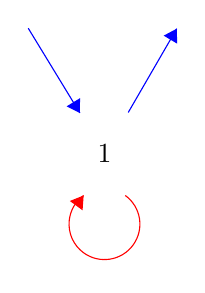
\begin{tikzpicture}[scale=0.2]
\tikzstyle{every node}+=[inner sep=0pt]

\draw (41.4,-30.4) node {$1$};

\draw [red] (42.723,-33.08) arc (54:-234:2.25);
\fill [red] (40.08,-33.08) -- (39.2,-33.43) -- (40.01,-34.02);

\draw [blue] (36.56,-22.46) -- (39.84,-27.84);
\fill [blue] (39.84,-27.84) -- (39.85,-26.9) -- (39,-27.42);

\draw [blue] (42.91,-27.81) -- (45.99,-22.49);
\fill [blue] (45.99,-22.49) -- (45.16,-22.93) -- (46.02,-23.44);
\end{tikzpicture}
\end{center}

Las aristas azules nos avisan de que el vértice debe tener una arista azul entrando y otra saliendo, sin embargo, no podemos asegurar que $1=1^b$. 
\vspace{0.4cm}



\item Vemos que el vértice $1$ ya cumple la relación $a^3=1$. La segunda relación no se verifica, por lo que procedemos a definir nuevas clases: $2:=1^b$ y $3:=2^b$, formando el siguiente triángulo cerrado de color azul:


\begin{center}
\begin{tikzpicture}[scale=0.2]
\tikzstyle{every node}+=[inner sep=0pt]
\draw (42.2,-44.7) node {$1$};
\draw (49.2,-33.3) node {$2$};
\draw (34.3,-33.3) node {$3$};

\draw [red] (43.523,-47.38) arc (54:-234:2.25);
\fill [red] (40.88,-47.38) -- (40,-47.73) -- (40.81,-48.32);

\draw [blue] (36.01,-35.77) -- (40.49,-42.23);
\fill [blue] (40.49,-42.23) -- (40.45,-41.29) -- (39.62,-41.86);

\draw [blue] (43.77,-42.14) -- (47.63,-35.86);
\fill [blue] (47.63,-35.86) -- (46.79,-36.28) -- (47.64,-36.8);

\draw [blue] (46.2,-33.3) -- (37.3,-33.3);
\fill [blue] (37.3,-33.3) -- (38.1,-33.8) -- (38.1,-32.8);

\draw [red] (46.04,-22.48) -- (48.36,-30.42);
\fill [red] (48.36,-30.42) -- (48.61,-29.51) -- (47.66,-29.79);

\draw [red] (35.12,-30.41) -- (37.38,-22.49);
\fill [red] (37.38,-22.49) -- (36.68,-23.12) -- (37.64,-23.39);

\draw [red] (50.25,-30.49) -- (53.25,-22.41);
\fill [red] (53.25,-22.41) -- (52.51,-22.99) -- (53.44,-23.34);

\draw [red] (29.59,-22.36) -- (33.11,-30.54);
\fill [red] (33.11,-30.54) -- (33.26,-29.61) -- (32.34,-30.01);

\end{tikzpicture}
\end{center}


La segunda relación $b^3=1$ ahora sí se verifica en el vértice $1$, pero no ocurre lo mismo con $(ab)^2=1$, obligándonos a definir $3:=2^a$ y completar el escaneo satisfactorio del vértice $1$.
De nuevo, las flechas rojas entrando y saliendo de los vértices $2$ y $3$ nos indican que el algoritmo no ha terminado y que se deben realizar nuevas definiciones para completar el grafo.




\begin{center}
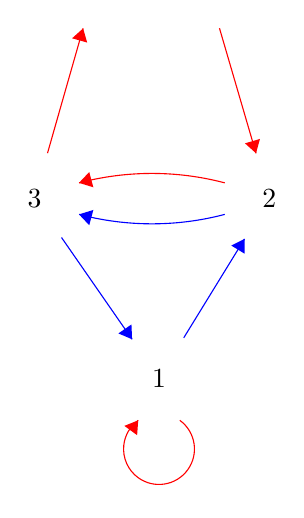
\begin{tikzpicture}[scale=0.2]
\tikzstyle{every node}+=[inner sep=0pt]
\draw (42.2,-44.7) node {$1$};
\draw (49.2,-33.3) node {$2$};
\draw (34.3,-33.3) node {$3$};

\draw [red] (43.523,-47.38) arc (54:-234:2.25);
\fill [red] (40.88,-47.38) -- (40,-47.73) -- (40.81,-48.32);

\draw [blue] (36.01,-35.77) -- (40.49,-42.23);
\fill [blue] (40.49,-42.23) -- (40.45,-41.29) -- (39.62,-41.86);

\draw [blue] (43.77,-42.14) -- (47.63,-35.86);
\fill [blue] (47.63,-35.86) -- (46.79,-36.28) -- (47.64,-36.8);

\draw [blue] (46.376,-34.301) arc (-75.22543:-104.77457:18.138);
\fill [blue] (37.12,-34.3) -- (37.77,-34.99) -- (38.03,-34.02);

\draw [red] (46.04,-22.48) -- (48.36,-30.42);
\fill [red] (48.36,-30.42) -- (48.61,-29.51) -- (47.66,-29.79);

\draw [red] (35.12,-30.41) -- (37.38,-22.49);
\fill [red] (37.38,-22.49) -- (36.68,-23.12) -- (37.64,-23.39);

\draw [red] (37.125,-32.299) arc (104.76944:75.23056:18.144);
\fill [red] (37.12,-32.3) -- (38.03,-32.58) -- (37.77,-31.61);
\end{tikzpicture}
\end{center}



\item Con el resto de vértices se sigue un proceso análogo al realizado con el vértice $1$. Ambos vértices $2$ y $3$, satisfacen $b^3=1$; sin embargo no ocurre lo mismo con el resto de relaciones, por lo que se procede a realizar las definiciones $4:=3^a$ y $2:=4^a$, obteniendo así el siguiente grafo:


\begin{center}
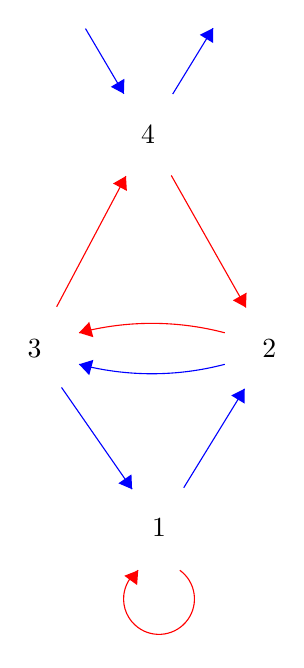
\begin{tikzpicture}[scale=0.2]
\tikzstyle{every node}+=[inner sep=0pt]
\draw (42.2,-44.7) node {$1$};
\draw (49.2,-33.3) node {$2$};
\draw (34.3,-33.3) node {$3$};
\draw (41.5,-19.7) node {$4$};

\draw [red] (43.523,-47.38) arc (54:-234:2.25);
\fill [red] (40.88,-47.38) -- (40,-47.73) -- (40.81,-48.32);

\draw [blue] (36.01,-35.77) -- (40.49,-42.23);
\fill [blue] (40.49,-42.23) -- (40.45,-41.29) -- (39.62,-41.86);

\draw [blue] (43.77,-42.14) -- (47.63,-35.86);
\fill [blue] (47.63,-35.86) -- (46.79,-36.28) -- (47.64,-36.8);

\draw [blue] (46.376,-34.301) arc (-75.22543:-104.77457:18.138);
\fill [blue] (37.12,-34.3) -- (37.77,-34.99) -- (38.03,-34.02);

\draw [red] (42.98,-22.31) -- (47.72,-30.69);
\fill [red] (47.72,-30.69) -- (47.76,-29.75) -- (46.89,-30.24);

\draw [red] (37.125,-32.299) arc (104.76944:75.23056:18.144);
\fill [red] (37.12,-32.3) -- (38.03,-32.58) -- (37.77,-31.61);

\draw [red] (35.7,-30.65) -- (40.1,-22.35);
\fill [red] (40.1,-22.35) -- (39.28,-22.82) -- (40.16,-23.29);

\draw [blue] (37.53,-12.98) -- (39.97,-17.12);
\fill [blue] (39.97,-17.12) -- (40,-16.17) -- (39.14,-16.68);

\draw [blue] (43.07,-17.14) -- (45.63,-12.96);
\fill [blue] (45.63,-12.96) -- (44.79,-13.38) -- (45.64,-13.9);

\end{tikzpicture}
\end{center}



\item Concluimos que la definición que falta debe ser $4:=4^b$, teniendo así un escaneo completo en todos los vértices y obteniendo un grafo completo, ya que cada vértice satisface  las tres relaciones, y dada una etiqueta $x \in X$, cada vértice tiene una arista saliendo y otra entrado con ésta.





\begin{center}
\begin{tikzpicture}[scale=0.2]
\tikzstyle{every node}+=[inner sep=0pt]
\draw (42.2,-44.7) node {$1$};
\draw (49.2,-33.3) node {$2$};
\draw (34.3,-33.3) node {$3$};
\draw (41.5,-20) node {$4$};
\draw [red] (43.523,-47.38) arc (54:-234:2.25);
\fill [red] (40.88,-47.38) -- (40,-47.73) -- (40.81,-48.32);

\draw [blue] (36.01,-35.77) -- (40.49,-42.23);
\fill [blue] (40.49,-42.23) -- (40.45,-41.29) -- (39.62,-41.86);

\draw [blue] (43.77,-42.14) -- (47.63,-35.86);
\fill [blue] (47.63,-35.86) -- (46.79,-36.28) -- (47.64,-36.8);

\draw [blue] (46.376,-34.301) arc (-75.22543:-104.77457:18.138);
\fill [blue] (37.12,-34.3) -- (37.77,-34.99) -- (38.03,-34.02);

\draw [red] (43,-22.6) -- (47.7,-30.7);
\fill [red] (47.7,-30.7) -- (47.73,-29.76) -- (46.86,-30.26);

\draw [red] (37.125,-32.299) arc (104.76944:75.23056:18.144);
\fill [red] (37.12,-32.3) -- (38.03,-32.58) -- (37.77,-31.61);

\draw [red] (35.73,-30.66) -- (40.07,-22.64);
\fill [red] (40.07,-22.64) -- (39.25,-23.1) -- (40.13,-23.58);

\draw [blue] (40.177,-17.32) arc (234:-54:2.25);
\fill [blue] (42.82,-17.32) -- (43.7,-16.97) -- (42.89,-16.38);
\end{tikzpicture}
\end{center}
\end{enumerate}

El vértice $1$ hace referencia a la clase $H \in G/H$. El vértice $2$ a la clase $Hb$, el vértice $3$ a la clase $Hb^{-1}=Hb^2$, y por último, el vértice $4$ a la clase $Hb^2a=Hba^2$.


Como consecuencia, se obtiene un algoritmo que resuelve el Problema de Palabras. Dos palabras $w, w'$ dadas en el alfabeto $X^{\pm 1}$ representan el mismo elemento si partiendo del vértice $1$ se sigue un recorrido en el que terminan en el mismo vértice. 


En ejemplos más complicados es de gran ayuda  usar una tabla de relator para cada relación que defina al grupo para así deducir nuevas definiciones y agilizar el proceso.   En la cabecera de cada tabla se coloca la relación, la primera posición de cada nueva fila hace referencia a cada clase de $G/H$. Por otro lado, como el recorrido debe acabar en el mismo vértice, la última posición de la fila debe coincidir con la primera. El resto de entradas de la tabla se deben rellenar si están definidas o se pueden deducir.


Para ilustrar el uso de estas tablas, repitamos el ejemplo anterior. En primer lugar, comenzamos definiendo la clase $1:=1^a$. Para reflejar esto en las tablas de relatores, se añade la clase $1$ como una nueva fila. Como el recorrido debe acabar en el mismo vértice, la última posición de cada fila también debe coincidir con la primera; en este caso, la clase $1$. En el resto de entradas se opera de forma parecida a una tabla de multiplicar.
\begin{align*}
\begin{array}{ccccccc}
& a && a && a \\
\hline
1 && 1 && 1 && 1
\end{array}
\qquad
\begin{array}{ccccccc}
& b && b && b \\
\hline
1&&  &&  && 1
\end{array}
\qquad
\begin{array}{ccccccccc}
& a && b && a && b\\
\hline
1 && 1 &&   &&  && 1
\end{array}
\end{align*}

La tabla de relator para $aaa$ ya está completa, pero no las otras dos, por lo que se siguen definiendo clases hasta completarlas.
Definimos $2:=1^b$ y, al hacer uso de una nueva clase, se añade una nueva fila y se completan las entradas cuyo valor conocemos:
\begin{align*}
\begin{array}{ccccccc}
& a && a && a \\
\hline
1 && 1 && 1 && 1 \\
2 &&   &&   && 2
\end{array}
\qquad
\begin{array}{ccccccc}
& b && b && b \\
\hline
1&& 2 &&  && 1 \\
2&&  &&  && 2
\end{array}
\qquad
\begin{array}{ccccccccc}
& a && b && a && b\\
\hline
1 && 1 && 2  &&  && 1 \\
2 &&  && 1  && 1 && 2
\end{array}
\end{align*}

De nuevo, $3:=2^b$ y se deduce que $3^b=1$. Como consecuencia, volvemos a añadir una nueva fila que hace referencia a la clase $3$. El escaneo es ahora satisfactorio en la tabla de relator $bbb$ para las $3$ clases.  
\begin{align*}
\begin{array}{ccccccc}
& a && a && a \\
\hline
1 && 1 && 1 && 1 \\
2 &&   &&   && 2 \\
3 &&   &&   && 3
\end{array}
\qquad
\begin{array}{ccccccc}
& b && b && b \\
\hline
1&& 2 && 3 && 1 \\
2&&3  && 1 && 2 \\
3&& 1 && 2 && 3
\end{array}
\qquad
\begin{array}{ccccccccc}
& a && b && a && b\\
\hline
1 && 1 && 2  && 3  && 1 \\
2 &&  && 1  && 1 && 2 \\
3 &&  &&    && 2 && 3
\end{array}
\end{align*}

Se sigue el mismo proceso realizado para el grafo de Schreier, definiendo las clases necesarias, $3:=2^a$, $4:=3^a$, $2:=4^a$ y $4:=4^b$, y completando así todas las tablas de relatores.
\begin{align*}
\begin{array}{ccccccc}
& a && a && a \\
\hline
1 && 1 && 1 && 1 \\
2 && 3  && 4  && 2 \\
3 && 4  &&  2 && 3 \\
4 &&  2 && 3  && 4
\end{array}
\qquad
\begin{array}{ccccccc}
& b && b && b \\
\hline
1&& 2 && 3 && 1 \\
2&&3  && 1 && 2 \\
3&& 1 && 2 && 3 \\
4&& 4 && 4 && 4
\end{array}
\qquad
\begin{array}{ccccccccc}
& a && b && a && b\\
\hline
1 && 1 && 2  && 3  && 1 \\
2 && 3 && 1  && 1 && 2 \\
3 && 4 &&  4  && 2 && 3 \\
4 && 2 &&  3  && 4 && 4
\end{array}
\end{align*}

Siguiendo el proceso que se realizó en el grafo de Schreier, no es dificil comprobar que las tablas de relatores anteriores son equivalentes al grafo obtenido.

Sabemos que el índice de $[G:H]$ coincide con el número de clases laterales, en total $4$. Podemos afirmar que $|H|=3$ ya que el generador $a$ de G no es el trivial. Por otro lado, aplicando el \textit{Teorema de Lagrange}:
\[
    |G|=[G:H]\cdot |H| = 4\cdot 3 = 12 .
\]


Una vez ejecutado el algoritmo sobre un grupo $G$ y un subgrupo $H \leq G$, obtenemos una tabla de clases de $G$ sobre $H$, que es equivalente a la acción de $G$ sobre las clases de $G/H$ por la multiplicación a la derecha. Podemos obtener de forma sencilla la representación por permutaciones del grupo $G$.


En nuestro ejemplo, tenemos: 
$ G :=\langle a,b \mid a^3, b^3, (ab)^2 \rangle$, $H=\langle a \rangle$ y $\Omega = \{1,2,3,4\}$. Definimos el homomorfismo $\varphi \colon G \to S(\Omega)$ del siguiente modo:
\begin{align*}
   \varphi \colon G &\longrightarrow S(\Omega)  \\
    a &\mapsto 
    \begin{pmatrix}
    1 & 2 & 3 & 4\\
    1 & 3 & 4 & 2 
    \end{pmatrix} = (234) \\
    b & \mapsto
    \begin{pmatrix}
    1 & 2 & 3 & 4\\
    2 & 3 & 1 & 4 
    \end{pmatrix} = 
    (123)
\end{align*}


Basta con observar en el grafo de Schreier el recorrido que sigue la acción para cada generador del grupo. En este ejemplo, tenemos que el grupo está generado por dos ciclos $(234)$ y $(123)$, que se conocen como generadores de Schreier, y claramente generan al grupo Alternado de orden $12$. Por tanto:
\[
    G \cong \langle(234),(123)\rangle = A_4 .
\]




\subsubsection{Coincidencias} \label{ident}

En el proceso de definición de las diferentes clases, se puede dar la situación de que dos clases distintas resultan ser la misma. Esto es lo que se conoce como \textit{coincidencia}, y cuando se detecta una de ellas, se ha de reemplazar el grafo $\Gamma$ por un grafo cociente que refleje dicha coincidencia. Esta es, quizás, la parte más complicada del algoritmo, y para ilustrarla, se resolverá el Ejemplo \ref{triv}.
Consideramos el grupo:
\[
    G = \langle X \mid R\rangle = \langle a,b \mid aba^{-1}b^{-1}b^{-1}, bab^{-1}a^{-1}a^{-1}  \rangle 
\]
y el subgrupo trivial $H=\{1\} \leq G $. Apliquemos el \textit{Algoritmo de Todd Coxeter}, usando el color \textcolor{red}{rojo} para representar la acción de $a$ y el \textcolor{blue}{azul} para la acción de $b$.


Se comienza con la clase $1$ y se realizan sucesivas definiciones hasta que el primer relator se escanee por completo:
    \[
    2:=1^a ,\quad 3:=2^b, \quad 4:=3^{a^{-1}}, \quad 5:=4^{b^{-1}} .
    \]
    A raíz de estas definiciones, se deduce que $1=5^{b^{-1}}$ y el grafo actual tiene forma de pentágono. 
    %Quizás es buena idea decir que por comodidad no se representan el resto de aristas que deben entrar y salir en
    %los vértices.
    

\begin{center}
\begin{tikzpicture}[scale=0.2]
\tikzstyle{every node}+=[inner sep=0pt]
\draw (35.2,-55.4) node {$1$};
\draw (42.7,-47.9) node {$2$};
\draw (37.3,-39.4) node {$3$};
\draw (27.3,-41.2) node {$4$};
\draw (25.8,-50.9) node {$5$};
\draw [red] (37.32,-53.28) -- (40.58,-50.02);
\fill [red] (40.58,-50.02) -- (39.66,-50.23) -- (40.37,-50.94);

\draw [blue] (41.09,-45.37) -- (38.91,-41.93);
\fill [blue] (38.91,-41.93) -- (38.92,-42.88) -- (39.76,-42.34);

\draw [red] (30.25,-40.67) -- (34.35,-39.93);
\fill [red] (34.35,-39.93) -- (33.47,-39.58) -- (33.65,-40.57);

\draw [blue] (26.26,-47.94) -- (26.84,-44.16);
\fill [blue] (26.84,-44.16) -- (26.23,-44.88) -- (27.21,-45.03);

\draw [blue] (32.49,-54.1) -- (28.51,-52.2);
\fill [blue] (28.51,-52.2) -- (29.01,-52.99) -- (29.44,-52.09);
\end{tikzpicture}
\end{center}
    
    
\vspace{0.3cm}

Se tendrán únicamente dos tablas de relatores, una para $a b  a^{-1} b^{-1} b^{-1}$ y otra para $b a b^{-1} a^{-1} a^{-1}$. A partir del grafo anterior, no es difícil ver que las tablas actuales son:

\begin{align*}
    \begin{array}{lllllllllll}
    & a && b && a^{-1} && b^{-1} && b^{-1}\\
    \hline
    1 && 2 && 3  && 4  && 5 && 1 \\
    2 &&  &&  &&  && 3 && 2\\
    3 &&  &&    &&  && 2 && 3\\
    4 && 3 &&    && 1 && 5 && 4\\
    5 && &&    &&  && 4 && 5
    \end{array}
    \hspace{0.7cm}
    \begin{array}{lllllllllll}
    & b && a && b^{-1} && a^{-1} && a^{-1}\\
    \hline
    1 && 5 &&   &&    && 2 && 1 \\
    2 && 3  &&   &&  &&  && 2\\
    3 &&  &&    &&  &&  && 3\\
    4 &&  &&    &&  && 3 && 4\\
    5 && 4 &&  3  && 2 && 1 && 5
    \end{array}
\end{align*}
    
En este punto, el vértice $1$ escanea satisfactoriamente el primer  relator. Para completar la primera fila del segundo relator, deducimos $1=5^a$ y definimos $6:=1^{b^{-1}}$. Pero esto último arroja también la deducción $6=2^a$. 

\begin{align*}
    \begin{array}{lllllllllll}
    & a && b && a^{-1} && b^{-1} && b^{-1}\\
    \hline
    1 && 2 &&  3 && 4   && 5 && 1 \\
    2 && 6 && 1  &&   && 3 && 2\\
    3 &&  &&    &&  &&  && 3\\
    4 && 3 &&    &&  &&   && 4\\
    5 && 1  &&  5   &&   && 4 && 5 \\
    6 &&   &&     &&    &&   && 6
    \end{array}
    \hspace{0.7cm}
    \begin{array}{lllllllllll}
    & b && a && b^{-1} && a^{-1} && a^{-1}\\
    \hline
    1 && 5 &&  1 && 6   && 2 && 1 \\
    2 && 3  &&   && 2 && 1 && 2\\
    3 &&  &&    &&  &&  && 3\\
    4 &&  &&    &&  && 3 && 4\\
    5 && 4 &&  3  && 2 && 1 && 5 \\
    6 && 1 &&  2  &&    && 2 && 6
    \end{array}
\end{align*}

El grafo de Schreier asociado al momento actual es el siguiente: 

\begin{center}
\begin{tikzpicture}[scale=0.2]
\tikzstyle{every node}+=[inner sep=0pt]
\draw (37.4,-37.1) node {$1$};
\draw (43.1,-27.9) node {$2$};
\draw (36,-19.2) node {$3$};
\draw (25.8,-23.7) node {$4$};
\draw (26.5,-34.3) node {$5$};
\draw (50.1,-38) node {$6$};


\draw [blue] (41.2,-25.58) -- (37.9,-21.52);
\fill [blue] (37.9,-21.52) -- (38.02,-22.46) -- (38.79,-21.83);

\draw [red] (28.54,-22.49) -- (33.26,-20.41);
\fill [red] (33.26,-20.41) -- (32.32,-20.28) -- (32.73,-21.19);

\draw [blue] (29.468,-33.928) arc (89.7581:61.42853:11.624);
\fill [blue] (29.47,-33.93) -- (30.27,-34.43) -- (30.27,-33.43);

\draw [blue] (26.3,-31.31) -- (26,-26.69);
\fill [blue] (26,-26.69) -- (25.55,-27.52) -- (26.55,-27.46);


\draw [red] (38.98,-34.55) -- (41.52,-30.45);
\fill [red] (41.52,-30.45) -- (40.67,-30.87) -- (41.52,-31.39);

\draw [blue] (47.11,-37.79) -- (40.39,-37.31);
\fill [blue] (40.39,-37.31) -- (41.16,-37.87) -- (41.23,-36.87);

\draw [red] (44.81,-30.37) -- (48.39,-35.53);
\fill [red] (48.39,-35.53) -- (48.35,-34.59) -- (47.52,-35.16);

\draw [red] (34.418,-37.362) arc (-91.71349:-117.09988:12.762);
\fill [red] (34.42,-37.36) -- (33.63,-36.84) -- (33.6,-37.84);
\end{tikzpicture}
\end{center}

\vspace{0.3cm}
A partir de aquí es cuando nos encontraremos \textit{coincidencias}. El proceso a seguir es el de reemplazar nuestro grafo de Schreier por un grafo cociente que refleje dicha coincidencia. Este nuevo grafo debe satisfacer las propiedades del grafo original (que cada vértice tenga exactamente una arista de cada color entrando y otra saliendo). Para llevar esto a cabo trabajaremos con relaciones de equivalencia, donde cada una de ellas estará representada por su elemento más pequeño.

Construiremos una función $p:\{1, \ldots ,6\} \longrightarrow \{ 1, \ldots ,6\}$ tal que $p(x)$ es equivalente a $x$ para todo $x$ y $p(x)\leq x$ para todo $x$. La igualdad se dará si, y sólo si,  $x$ es el representante de su clase de equivalencia.

En resumen, dada una coincidencia, se deberá eliminar el vértice que tenga un mayor valor en su clase de equivalencia  y transferir todas las aristas que entran y salen al vértice que tenga un menor valor en dicha clase. Por otro lado, si estamos ante una situación en la que se produzcan coincidencias consecutivas, se hará uso de una cola (\textit{queue}) para indicar aquellas clases que se han eliminado pero aún deben ser procesadas.

Por ejemplo, la segunda fila del primer relator se escanea por completo y nos da la deducción $3=5^{b^{-1}}$; sin embargo, cuando añadimos una arista de color azul desde $3\rightarrow5$, nos damos cuenta que el $5$ recibe una arista de ese mismo color del vértice $1$; por ello, obtenemos la coincidencia $3=1$.
Para empezar, definamos $p(3):=1$ y $p(x):=x$ si $x \not = 3$. El grafo cociente tiene ahora $5$ vértices: $1,2,4,5$ y $6$.


Consideramos las aristas que salen y entran de $3$:
\begin{itemize}
    \item \texttt{Arista azul $2\rightarrow 3$}: se convierte en una arista azul $2\rightarrow1$ en el cociente. Sin embargo, el vértice $1$ ya recibe una arista azul de $6$, luego volvemos a obtener una coincidencia $6=2$. Por orden, se borra la arista $2 \rightarrow 3$, se redefine $p(6):=2$ (para reflejar que $6$ es equivalente a $2$) y se añade $6$ a la cola de clases.
    
    \item \texttt{Arista roja $4\rightarrow3$}. Al intentar añadir una arista roja de $4\rightarrow1$ nos encontramos con que a $1$ ya le llega una arista de este color desde $5$. Se trata de una coincidencia $5=4$. De nuevo, y por orden, se borra la arista roja $4\rightarrow3$, se define $p(5):=4$ ($5$ es equivalente a $4$), se añade $5$ a la cola para procesarlo más adelante y se borra el vértice $3$.
\end{itemize}

Procesamos ahora las aristas que entran y salen del vértice $6$:
\begin{itemize}
    \item \texttt{Arista azul $6\rightarrow1$}: como $6$ es equivalente a $2$, esta arista se convierte en una arista de $2\rightarrow1$.
    \item \texttt{Arista roja $2\rightarrow6$}:  pasa a ser una arista roja que sale y entra del $2$.
\end{itemize}

El siguiente vértice que se encontraba en la cola era $5$, cuyas aristas deben procesarse:
\begin{itemize}
    \item \texttt{Arista roja $5 \rightarrow 1$}: se convierte en una arista roja $4\rightarrow1$.
    \item \texttt{Aristas azules $1 \rightarrow 5$ y $5 \rightarrow 4$}: ambas pasan a ser una arista azul $1 \rightarrow 4$.
\end{itemize}
    Como ya se han procesado todas las aristas de los vértices $4$ y $6$, se pueden eliminar, obteniendo el siguiente grafo, que contiene $3$ vértices: $1,2$ y $4$:
    
    \begin{center}
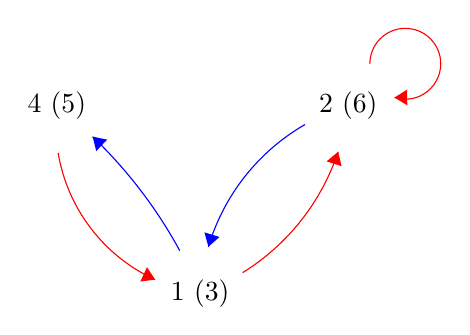
\begin{tikzpicture}[scale=0.2]
\tikzstyle{every node}+=[inner sep=0pt]
\draw (36.1,-33.3) node {$1\mbox{ }(3)$};
\draw (45.5,-21.4) node {$2\mbox{ }(6)$};
\draw (27,-21.4) node {$4\mbox{ }(5)$};

\draw [red] (44.857,-24.325) arc (-18.39525:-58.21629:14.355);
\fill [red] (44.86,-24.32) -- (44.13,-24.93) -- (45.08,-25.24);
\draw [blue] (36.624,-30.353) arc (163.46869:119.91976:13.329);
\fill [blue] (36.62,-30.35) -- (37.33,-29.73) -- (36.37,-29.44);

\draw [blue] (29.268,-23.362) arc (46.242:28.56871:29.647);
\fill [blue] (29.27,-23.36) -- (29.5,-24.28) -- (30.19,-23.55);

\draw [red] (33.236,-32.441) arc (-114.63987:-170.54942:10.811);
\fill [red] (33.24,-32.44) -- (32.72,-31.65) -- (32.3,-32.56);
\draw [red] (46.875,-18.747) arc (180.34746:-107.65254:2.25);
\fill [red] (48.44,-20.88) -- (49.25,-21.37) -- (49.24,-20.37);
\end{tikzpicture}
\end{center}

Sin embargo, el vértice $2$ tiene dos aristas rojas entrando, por lo que se obtiene la coincidencia $2=1$. Ahora bien, se redefine $p(2):=1$ para indicar que el vértice $2$ es equivalente a $1$.

\begin{center}
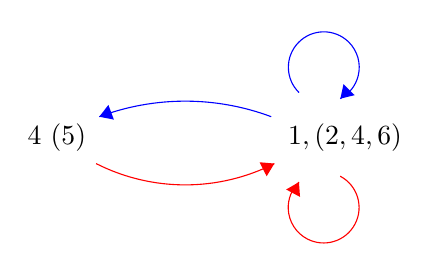
\begin{tikzpicture}[scale=0.2]
\tikzstyle{every node}+=[inner sep=0pt]
\draw (45.3,-21.4) node {$1,(2,4,6)$};
\draw (27,-21.4) node {$4\mbox{ }(5)$};

\draw [blue] (29.692,-20.086) arc (110.51126:69.48874:15.578);
\fill [blue] (29.69,-20.09) -- (30.62,-20.27) -- (30.27,-19.34);

\draw [red] (40.812,-23.063) arc (-63.10491:-116.89509:12.516);
\fill [red] (40.81,-23.06) -- (39.87,-22.98) -- (40.32,-23.87);

\draw [blue] (42.378,-18.557) arc (225.69534:-62.30466:2.25);
\fill [blue] (45,-18.94) -- (45.91,-18.72) -- (45.2,-18.02);

\draw [red] (44.99,-23.865) arc (62.16578:-225.83422:2.25);
\fill [red] (42.37,-24.24) -- (41.56,-24.71) -- (42.44,-25.18);
\end{tikzpicture}
\end{center}

En el vértice $1$ entran dos aristas de color rojo y salen otras dos de color azul, luego se redefine $p(4):=1$ al obtener la coincidencia $4=1$. Siguiendo el mismo proceso para las aristas de $4$, se obtiene finalmente que el grafo cociente es el vértice $1$. El \textit{Algoritmo de Todd Coxeter} ha terminado y prueba que $G$ es el grupo trivial.


\begin{center}
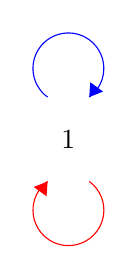
\begin{tikzpicture}[scale=0.2]
\tikzstyle{every node}+=[inner sep=0pt]
\draw (40.1,-23.5) node {$1$};
\draw [blue] (38.777,-20.82) arc (234:-54:2.25);
\fill [blue] (41.42,-20.82) -- (42.3,-20.47) -- (41.49,-19.88);
\draw [red] (41.423,-26.18) arc (54:-234:2.25);
\fill [red] (38.78,-26.18) -- (37.9,-26.53) -- (38.71,-27.12);
\end{tikzpicture}
\end{center}





\blankpage


